\chapter{HASIL DAN PEMBAHASAN} \label{cha:4-HasilDanPembahasan}

\section{Hasil Pemelajaran Model} \label{sec:4-PersiapanPengujian}

Pemelajaran model yang dilakukan selama sepuluh \textit{epochs} menunjukkan bahwa kesalahan model
dalam mengestimasi pose tiga dimensi berkurang dalam setiap \textit{epoch}. \text{Learning rate}
yang dibagi dua dalam setiap \textit{epoch} mempengaruhi pemelajaran model dimana penyesuaian model
semakin teliti. Adaptasi bobot model terjadi secara drastis pada \textit{epoch} 0 sampai dengan
\textit{epoch} 3. \textit{Epoch} 4 dan seterusnya menggunakan \textit{learning rate} yang semakin
kecil sehingga model semakin teliti dalam melakukan adaptasi. Grafik pemelajaran model dapat dilihat
pada gambar~\ref{fig:pelatihan}.

\begin{figure}[htbp]
    \begin{center}
        \fbox{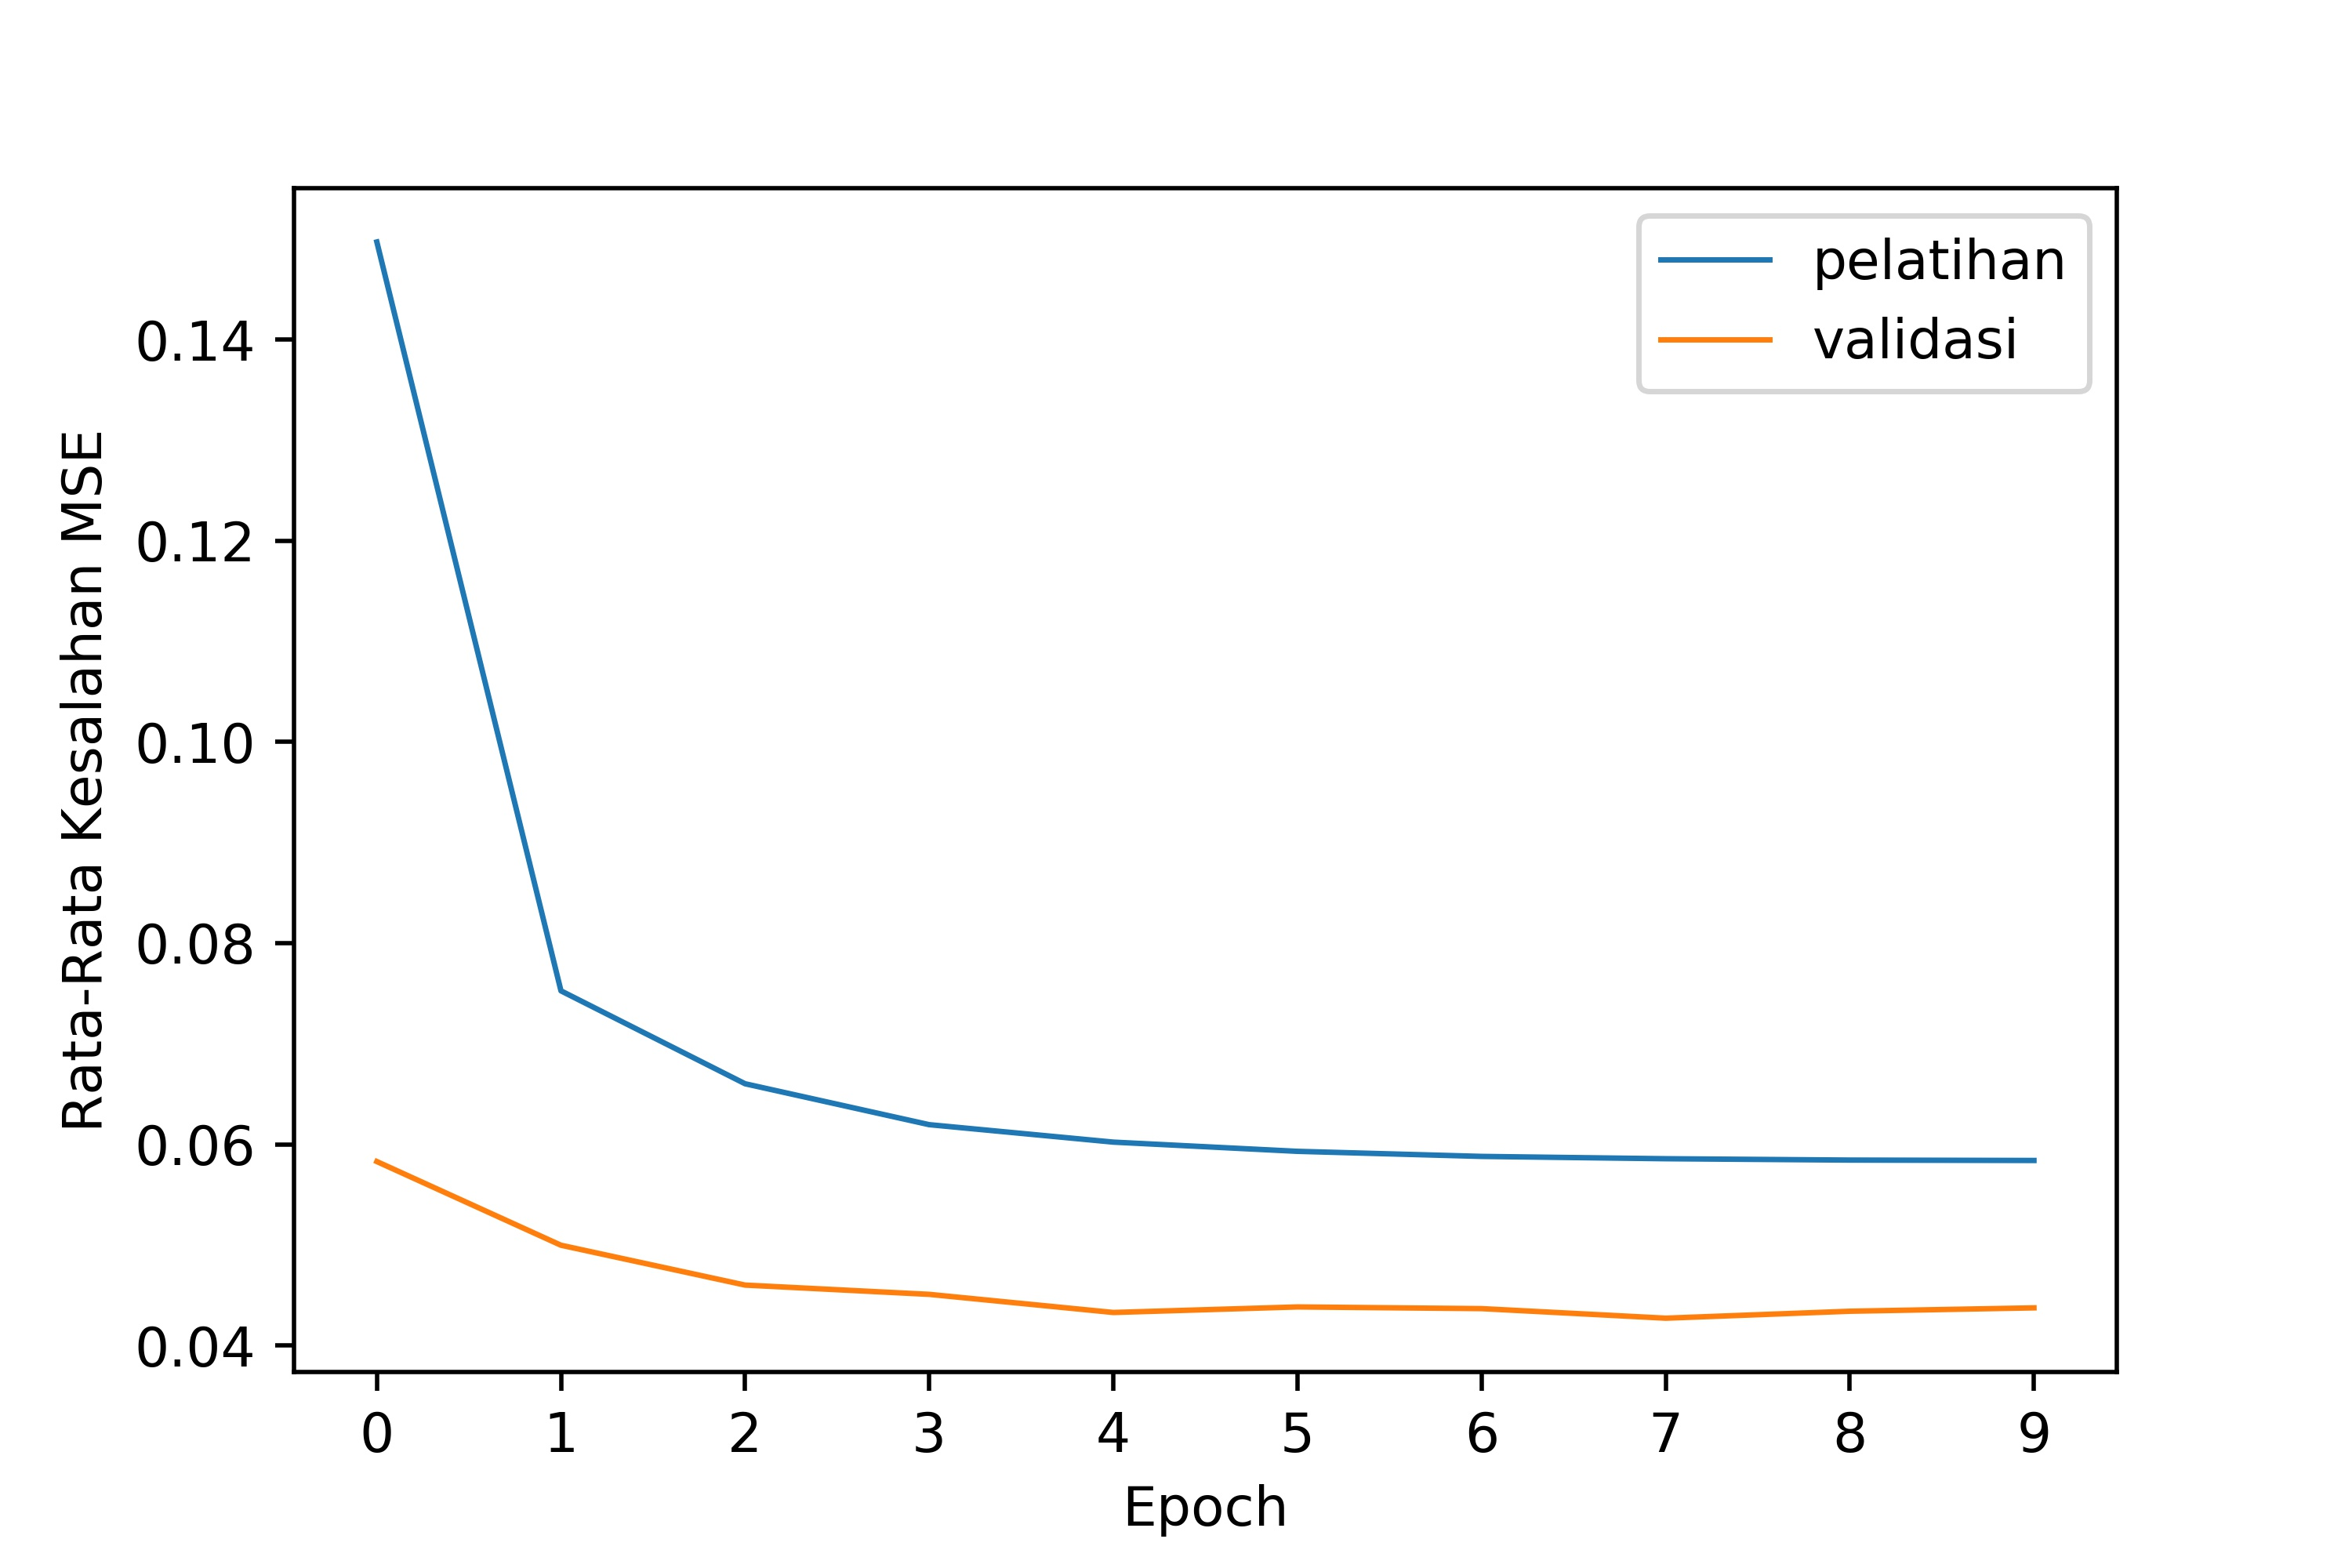
\includegraphics[width=11.9cm]{bab4/gambar/pelatihan.jpg}}
    \end{center}
    \vspace{-20pt}
    \captionsetup{labelfont=bf, textfont=bf}
    \caption{Grafik Pemelajaran Model}
    \vspace{-10pt}
    \captionsetup{labelfont=md, textfont=md}
    % \caption*{Sumber: sumber}
    % \caption*{Sumber: nama(2019)}
    \label{fig:pelatihan}
\end{figure}

\section{Analisis Uji Coba Aplikasi} \label{sec:4-PersiapanPengujian}

Inferensi yang bagus akan terjadi apabila langkah-langkah pada tahapan uji coba tidak mengalami
kesalahan. Kualitas gambar dan pose yang tidak cacat juga mempengaruhi proses dari awal hingga akhir.
Prapemrosesan gambar pada data inferensi yang tepat memudahkan OpenPose dalam mencari titik kunci
pose dua dimensi secara lengkap. Titik kunci OpenPose yang lengkap kemudian memenuhi syarat untuk
dikonversi menjadi spesifikasi yang diinginkan. Informasi tersebut kemudian diteruskan ke model
untuk mendapatkan titik kunci pose tiga dimensi.
% Rangkaian langkah-langkah yang baik menghasilkan
% pose tiga dimensi yang realistis seperti pada gambar~\ref{fig:bro75}.

% \begin{figure}[htbp]
%     \begin{center}
%         \fbox{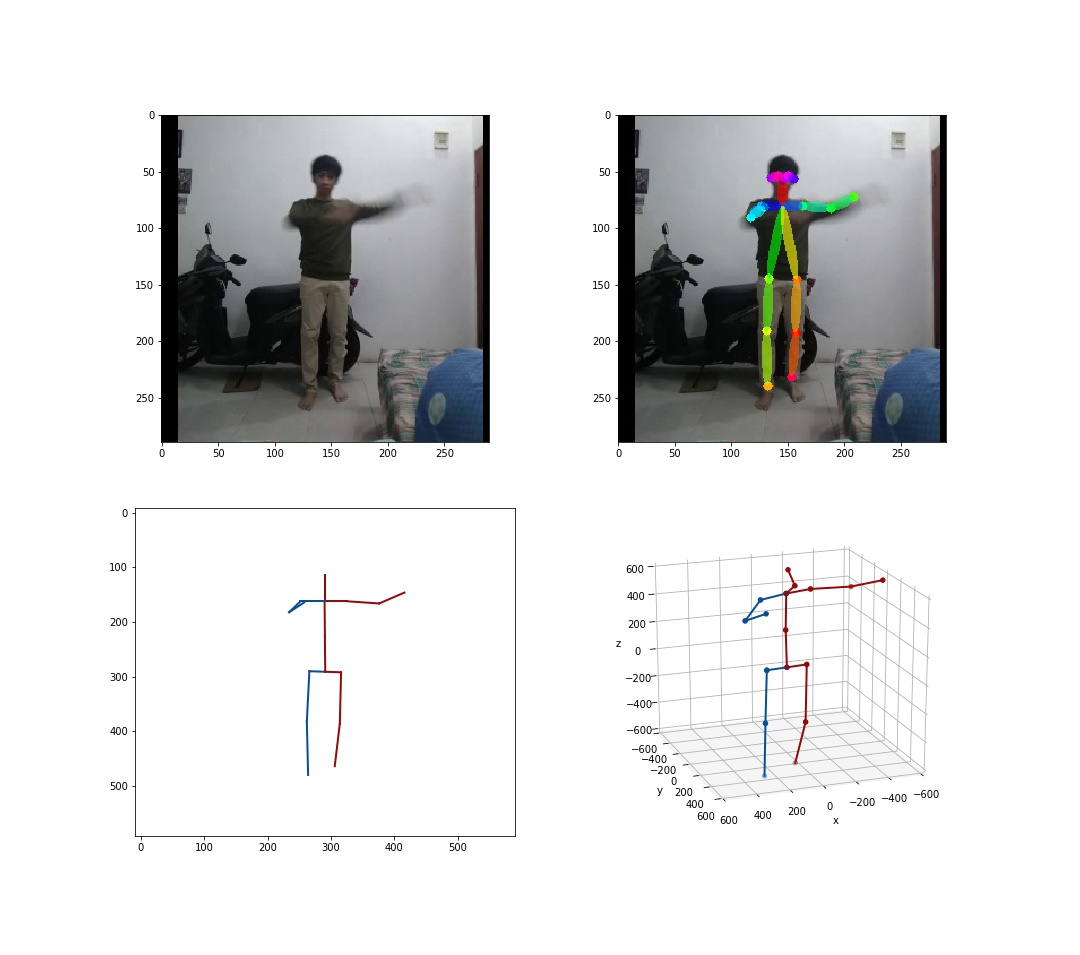
\includegraphics[width=11.9cm]{bab4/gambar/bro75.jpg}}
%     \end{center}
%     \vspace{-20pt}
%     \captionsetup{labelfont=bf, textfont=bf}
%     \caption{Inferensi Tepat}
%     \vspace{-10pt}
%     \captionsetup{labelfont=md, textfont=md}
%     % \caption*{Sumber: sumber}
%     % \caption*{Sumber: nama(2019)}
%     \label{fig:bro75}
% \end{figure}

Kualitas pose yang cacat menghasilkan estimasi pose tiga dimensi yang cacat. Oklusi pose pada gambar
dua dimensi dapat menghilangkan suatu bagian tubuh. Hilangnya bagian ini dari gambar menyebabkan
kesalahan pada langkah-langkah selanjutnya. Titik kunci lengan kanan hilang ketika pose lengan
mengarah lurus ke lensa kamera sehingga terjadi oklusi. Hal ini menyebabkan OpenPose tidak dapat
menemukan titik kunci lengan kanan dan memberi nilai nol pada titik kunci tersebut. Proses konversi
dan inferensi titik kunci tiga dimensi juga menghasilkan pose yang tidak realistis. Inferensi pose
hilang yang diakibatkan oklusi dapat dilihat pada gambar~\ref{fig:bro76}.

\begin{figure}[htbp]
    \begin{center}
        \fbox{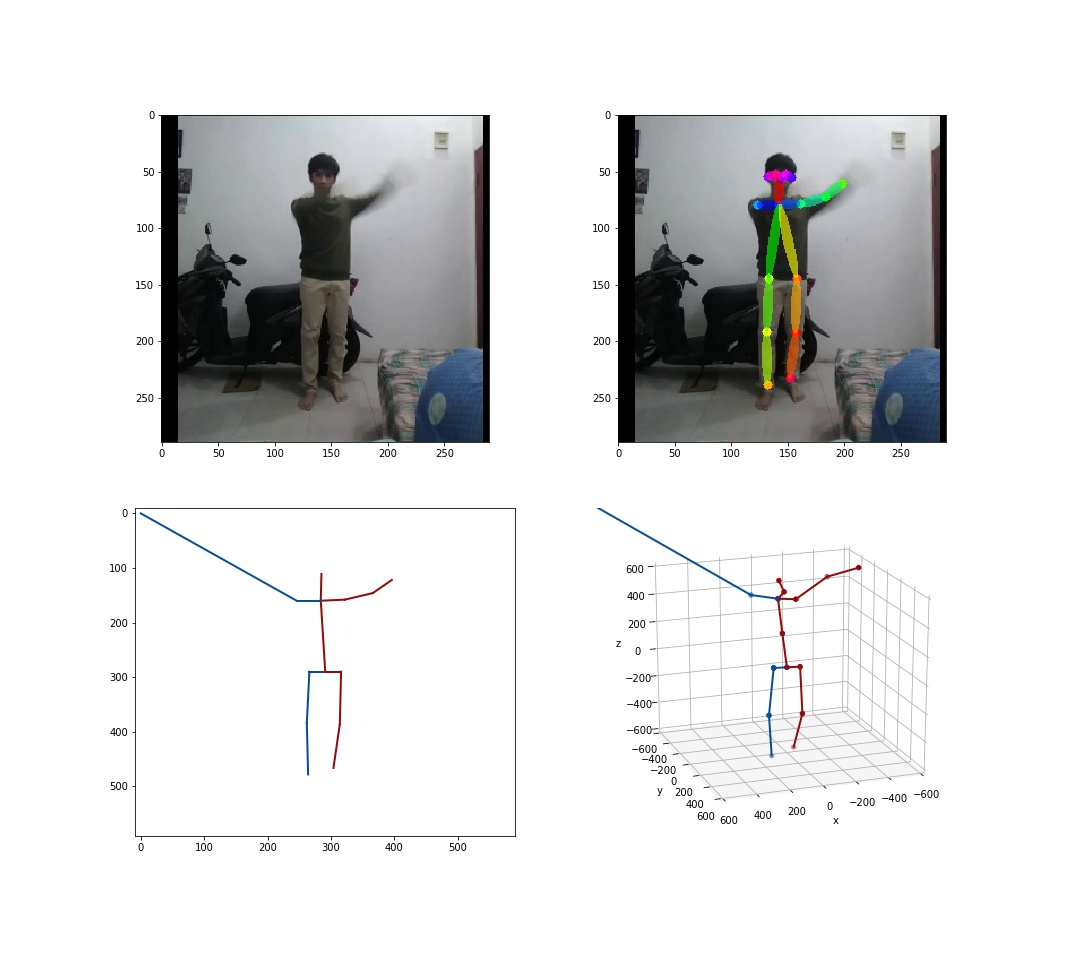
\includegraphics[width=11.9cm]{bab4/gambar/bro76.jpg}}
    \end{center}
    \vspace{-20pt}
    \captionsetup{labelfont=bf, textfont=bf}
    \caption{Inferensi Pose Hilang}
    \vspace{-10pt}
    \captionsetup{labelfont=md, textfont=md}
    % \caption*{Sumber: sumber}
    % \caption*{Sumber: nama(2019)}
    \label{fig:bro76}
\end{figure}

\pagebreak

Kesalahan juga dapat terjadi pada proses inferensi titik kunci. Apabila OpenPose mengeluarkan
\textit{output} yang ambigu dimana terdapat titik kunci yang dianggap sebagai bagian dari tubuh manusia.
OpenPose menghasilkan titik kunci ganda yang tidak sesuai dengan spesifikasi yang diperlukan meskipun
berhasil mendeteksi pose secara lengkap.
Hasil keluaran yang tidak sesuai dengan spesifikasi model mengakibatkan estimasi pose tiga dimensi yang rusak.
Inferensi pose yang mengalami kesalahan deteksi dapat dilihat pada gambar~\ref{fig:bro131}.

\begin{figure}[htbp]
    \begin{center}
        \fbox{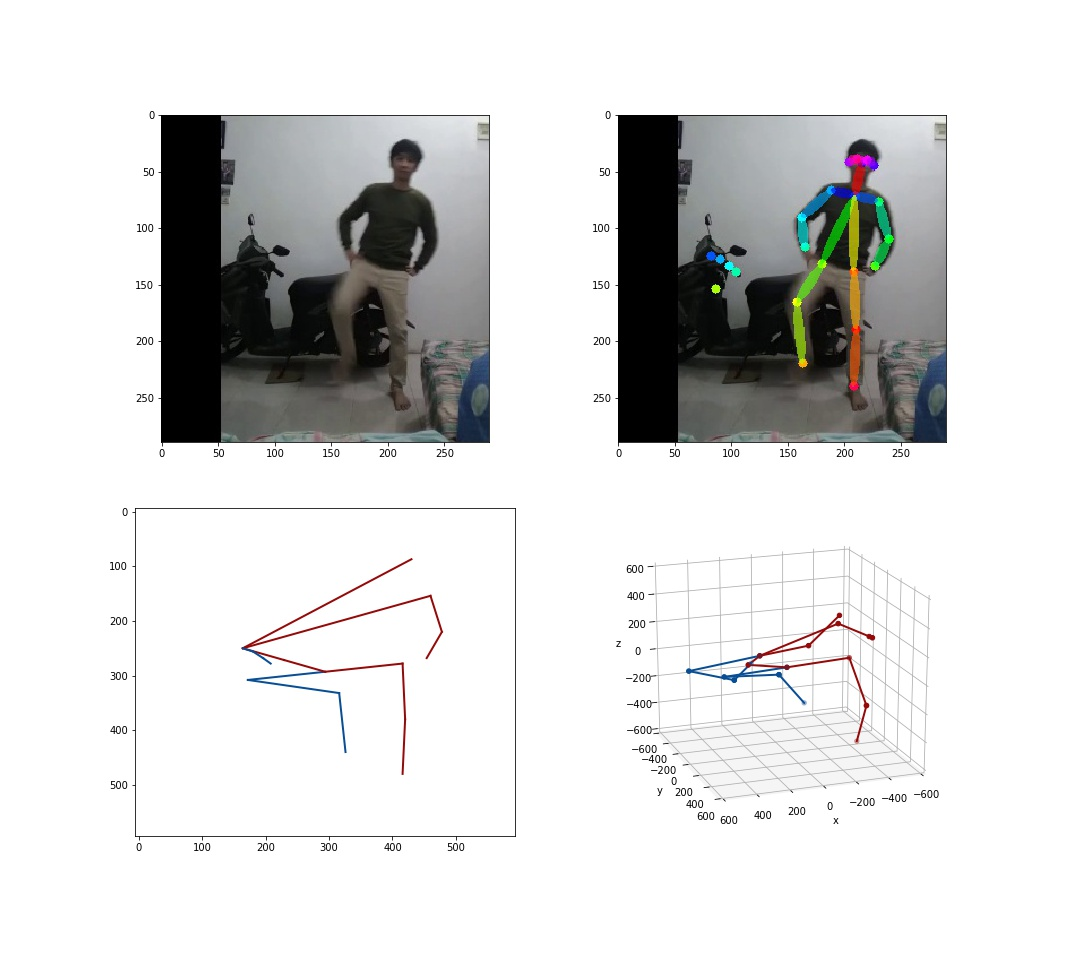
\includegraphics[width=11.9cm]{bab4/gambar/bro131.jpg}}
    \end{center}
    \vspace{-20pt}
    \captionsetup{labelfont=bf, textfont=bf}
    \caption{Kesalahan Deteksi}
    \vspace{-10pt}
    \captionsetup{labelfont=md, textfont=md}
    % \caption*{Sumber: sumber}
    % \caption*{Sumber: nama(2019)}
    \label{fig:bro131}
\end{figure}

\pagebreak

Kesalahan estimasi pose tiga dimensi yang terjadi pada masukkan video uji coba dapat dianalisis
lebih mendalam.
Setiap titik kunci memiliki peran kontribusi terhadap estimasi pose secara keseluruhan. Analisis
setiap titik kunci secara tersendiri dilakukan dengan
pemberian nama kode.
Kode-kode terdiri dari lima belas titik kunci yang diwakilkan dengan kode huruf kapital terurut seperti pada
tabel \ref{tab:definisititikkunci} untuk mempermudah analisis.

\begin{table}[htbp]
    \captionsetup{labelfont=bf, textfont=bf}
    \caption{Definisi Titik Kunci}
    \label{tab:definisititikkunci}
    \vspace{-20pt}
    \begin{center}
        \begin{tabular}{|c|c|l|}
            \hline
            \textbf{No.} & \textbf{Kode} & \hspace{2cm}\textbf{Titik Kunci} \\ \hline
            1            & A             & Pinggang                         \\ \hline
            2            & B             & Paha Kanan                       \\ \hline
            3            & C             & Lutut Kanan                      \\ \hline
            4            & D             & Pergelangan Kaki Kanan           \\ \hline
            5            & E             & Paha Kiri                        \\ \hline
            6            & F             & Lutut Kiri                       \\ \hline
            7            & G             & Pergelangan Kaki Kiri            \\ \hline
            8            & H             & Leher                            \\ \hline
            9            & I             & Bahu Kanan                       \\ \hline
            10           & J             & Siku Kanan                       \\ \hline
            11           & K             & Pergelangan Tangan Kanan         \\ \hline
            12           & L             & Bahu Kiri                        \\ \hline
            13           & M             & Siku Kiri                        \\ \hline
            14           & N             & Pergelangan Tangan Kiri          \\ \hline
            15           & O             & Kepala                           \\ \hline
        \end{tabular}
    \end{center}
    \vspace{-10pt}
\end{table}

Hasil uji akurasi estimasi pose untuk setiap pose ditampilkan pada tabel \ref{tab:hasilujiakurasiestimasipose}.
Setiap kode titik kunci yang diisi dengan tanda "\checkmark" mewakili kesalahan estimasi yang terjadi
pada titik kunci tersebut.
Keberadaan kuantitas kesalahan tersebut dikalikan dengan banyaknya jumlah frame untuk mendapatkan
total jumlah kesalahan. Kuantitas kesalahan setiap titik kunci juga dijumlahkan sehingga pada akhirnya
didapatkan persentase kesalahan estimasi setiap titik kunci terhadap kesalahan estimasi keseluruhan.

\pagebreak

\begin{table}[htbp]
    \captionsetup{labelfont=bf, textfont=bf}
    \caption{Hasil Uji Akurasi Estimasi Pose}
    \label{tab:hasilujiakurasiestimasipose}
    \vspace{-20pt}
    \begin{center}
        \tiny
        \begin{tabular}{|l|c|c|c|c|c|c|c|c|c|c|c|c|c|c|c|c|}
            \hline
            \textbf{No.}   & \multicolumn{16}{c|}{\textbf{Kode Titik Kunci}}                                                                                                                                                                                                      \\
            \cline{2-17}
            \textbf{Frame} & \textbf{A}                                      & \textbf{B} & \textbf{C} & \textbf{D} & \textbf{E} & \textbf{F} & \textbf{G} & \textbf{H} & \textbf{I} & \textbf{J} & \textbf{K} & \textbf{L} & \textbf{M} & \textbf{N} & \textbf{O} & \textbf{Jlh} \\ \hline
            1-77           &                                                 &            &            &            &            &            &            &            &            &            &            &            &            &            &            & 0            \\ \hline
            78-82          &                                                 &            & \checkmark & \checkmark &            & \checkmark & \checkmark &            &            &            &            &            &            &            &            & 20           \\ \hline
            83-86          &                                                 &            &            &            &            &            &            &            &            & \checkmark & \checkmark &            &            &            &            & 8            \\ \hline
            87-89          &                                                 &            &            &            &            &            &            &            &            &            &            &            &            &            &            & 0            \\ \hline
            90             &                                                 &            & \checkmark &            &            &            &            &            &            &            &            &            &            &            &            & 1            \\ \hline
            91-92          &                                                 &            &            &            &            &            &            &            &            &            &            &            &            &            &            & 0            \\ \hline
            93             &                                                 &            & \checkmark &            &            &            &            &            &            &            &            &            &            &            &            & 1            \\ \hline
            94-97          &                                                 &            &            &            &            &            &            &            &            &            &            &            &            &            &            & 0            \\ \hline
            98-100         &                                                 &            &            &            &            &            &            &            &            &            &            &            & \checkmark & \checkmark &            & 6            \\ \hline
            101            &                                                 &            &            &            &            &            & \checkmark &            &            &            &            &            &            &            &            & 1            \\ \hline
            102-104        &                                                 &            &            &            &            &            &            &            &            &            &            &            &            &            &            & 0            \\ \hline
            105            &                                                 &            &            &            &            &            & \checkmark &            &            &            &            &            &            &            &            & 1            \\ \hline
            106            &                                                 &            &            &            &            &            &            &            &            &            &            &            &            &            &            & 0            \\ \hline
            107            &                                                 &            &            &            &            &            &            &            &            &            &            &            &            & \checkmark &            & 1            \\ \hline
            108-122        &                                                 &            &            &            &            &            &            &            &            &            &            &            &            &            &            & 0            \\ \hline
            123-124        &                                                 &            &            &            &            &            &            & \checkmark & \checkmark & \checkmark & \checkmark & \checkmark & \checkmark & \checkmark & \checkmark & 16           \\ \hline
            125            &                                                 &            &            &            &            &            &            &            &            &            &            &            &            &            &            & 0            \\ \hline
            126            &                                                 &            &            & \checkmark &            &            &            &            &            &            &            &            &            &            &            & 1            \\ \hline
            127-129        &                                                 &            &            &            &            &            &            &            &            &            &            &            &            &            &            & 0            \\ \hline
            130            &                                                 &            &            &            &            &            &            &            &            &            & \checkmark &            &            &            &            & 1            \\ \hline
            131-132        & \checkmark                                      & \checkmark & \checkmark & \checkmark & \checkmark & \checkmark & \checkmark & \checkmark & \checkmark & \checkmark & \checkmark & \checkmark & \checkmark & \checkmark & \checkmark & 30           \\ \hline
            133-134        &                                                 &            & \checkmark & \checkmark &            &            &            &            &            &            &            &            &            &            &            & 4            \\ \hline
            135-137        &                                                 &            &            &            &            &            &            &            &            &            &            &            &            &            &            & 0            \\ \hline
            138            &                                                 &            &            & \checkmark &            &            &            &            &            &            &            &            &            &            &            & 1            \\ \hline
            139-140        &                                                 &            &            &            &            &            &            &            &            &            & \checkmark &            &            &            &            & 2            \\ \hline
            141-169        &                                                 &            &            &            &            &            &            &            &            &            &            &            &            &            &            & 0            \\ \hline
            170-173        &                                                 &            &            &            &            &            &            &            &            &            &            &            & \checkmark & \checkmark &            & 8            \\ \hline
            174-190        &                                                 &            &            &            &            &            &            &            &            &            &            &            &            &            &            & 0            \\ \hline
            191-192        &                                                 &            &            &            &            &            &            &            &            &            &            &            &            &            & \checkmark & 2            \\ \hline
            193-196        &                                                 &            &            &            &            &            &            &            &            &            &            & \checkmark & \checkmark & \checkmark & \checkmark & 16           \\ \hline
            197-201        & \checkmark                                      & \checkmark & \checkmark & \checkmark & \checkmark & \checkmark & \checkmark & \checkmark & \checkmark & \checkmark & \checkmark & \checkmark & \checkmark & \checkmark & \checkmark & 75           \\ \hline
            202-223        &                                                 &            &            &            &            &            &            &            &            &            &            &            &            &            &            & 0            \\ \hline
            224-232        &                                                 &            &            &            &            &            &            &            &            &            &            &            & \checkmark & \checkmark & \checkmark & 27           \\ \hline
            233-309        &                                                 &            &            &            &            &            &            &            &            &            &            &            &            &            &            & 0            \\ \hline
            310-359        &                                                 &            &            &            &            &            &            &            &            &            &            &            &            &            &            & 0            \\ \hline
            360-362        & \checkmark                                      &            &            &            &            &            &            & \checkmark & \checkmark & \checkmark & \checkmark & \checkmark & \checkmark & \checkmark & \checkmark & 27           \\ \hline
            363-374        &                                                 &            &            &            &            &            &            &            &            &            &            &            &            &            &            & 0            \\ \hline
            \hline
            Total          & 10                                              & 7          & 16         & 16         & 7          & 12         & 14         & 12         & 12         & 16         & 19         & 16         & 32         & 33         & 27         & 249          \\ \hline
            Persen         & 4.02                                            & 2.81       & 6.43       & 6.43       & 2.81       & 4.82       & 5.62       & 4.82       & 4.82       & 6.43       & 7.63       & 6.43       & 12.85      & 13.25      & 10.84      & \%           \\\hline %5\% \\ \hline
        \end{tabular}
    \end{center}
\end{table}

Nilai akurasi dan kesalahan estimasi titik kunci berbeda-beda pada setiap titik kunci.
Titik kunci B dan C yang mewakili titik paha kanan dan lutut kanan secara berurut merupakan
titik dengan hasil estimasi paling akurat. Kedua titik tersebut salah diestimasi sebanyak tujuh kali
dari total dua ratus empat puluh sembilan kesalahan estimasi. Persentase kesalahan akhir
bernilai dua koma delapan puluh satu persen dari total kesalahan estimasi.

Titik kunci N yang mewakili titik kunci pergelangan tangan kiri merupakan titik dengan hasil estimasi
paling tidak akurat. Titik tersebut salah diestimasi sebanyak tiga puluh tiga kali dari total
dua ratus empat puluh sembilang kesalahan estimasi. Hasil akhir kesalahan pada titik ini bernilai
tiga belas koma dua puluh lima persen dari keseluruhan kesalahan estimasi.